\documentclass[a4paper,12pt]{article}

%\documentclass[11pt,a4paper,oneside]{report}
\usepackage[top=0.75in, bottom=0.75in, left=1.25in, right=0.75in]{geometry}
\usepackage[pdftex]{graphicx}
\usepackage[T1]{fontenc}
\usepackage{fancyhdr}
\usepackage{algorithm}
\usepackage{algorithmic}
\usepackage{amssymb}
\usepackage{amsmath}
\usepackage{subfigure}
\setcounter{tocdepth}{3}
\usepackage{graphicx}
\usepackage{enumerate}
\usepackage{verbatim}

\newcommand{\HRule}{\rule{\linewidth}{0.5mm}}

\makeatletter
\newcommand{\rmnum}[1]{\romannumeral #1}
\newcommand{\Rmnum}[1]{\expandafter\@slowromancap\romannumeral #1@}
\makeatother

\begin{document}

\renewcommand*\rmdefault{ppl}\normalfont\upshape
\renewcommand{\headrulewidth}{0.5pt}
\renewcommand{\footrulewidth}{0.5pt}

\pagestyle{fancy}

%%%%%%%%%%%%%%%%%%%%%%%%%%%%%%%%%%%%%%%%%%%%%%%%%%%%TITLE PAGE%%%%%%%%%%%%%%%%%%%%%%%%%%%%%%%%%%%%%%%%%%%%%%%%%%%%%%%%%%%%%%%%%%%%%%%%%%%

\begin{titlepage}
\begin{center}
\newpage


\includegraphics[width=0.3\textwidth]{./logo}\\[2cm]    
%\textsc{\LARGE PES Institute of Technology}\\[1.5cm]

\textsc{\Large  \Rmnum{6} Semester Special Topic}\\[0.5cm]

\HRule \\[0.4cm]
{ \huge \bfseries A Bidirectional Search Algorithm in Power Law Networks}\\[0.4cm]
\HRule \\[1.5cm]

\vspace{1in}
% Title

% Author and supervisor
\begin{minipage}{0.4\textwidth}
\begin{flushleft} \large
\emph{By:}\\
Vijay Mahantesh S M\\
-1PI09CS118\\
Vijesh M\\
-1PI09CS119
\end{flushleft}
\end{minipage}
\begin{minipage}{0.4\textwidth}
\begin{flushright} \large
\emph{Guided By:} \\
Dr. Kavi Mahesh\\
Professor \\
Computer Science Dept\\
PESIT, Bangalore 
\end{flushright}
\end{minipage}

%\vfill
% Bottom of the page
\end{center}
\end{titlepage}
%%%%%%%%%%%%%%%%%%%%%%%%%%%%%%%%%%%%%%%%%%%%%%%%%%%%END TITLE PAGE%%%%%%%%%%%%%%%%%%%%%%%%%%%%%%%%%%%%%%%%%%%%%%%%%%%%%%%%%%%%%%%%%%%%%%
\begin{center}

\vspace{15in}


\includegraphics[width=0.3\textwidth]{./logo}\\[2cm]    

\includegraphics[width=0.3\textwidth]{./certificate-text.png}\\[2cm]
\normalfont
\rmfamily{\Large{This is to certify that Vijay Mahantesh SM (1PI09CS118) and Vijesh M (1PI09CS119) have satisfactorily completed the Special Topic Project prescribed by PES Institute of Technology (Autonomous Institute under VTU) in the year 2012 (January - May).}}\\[4cm]
\begin{minipage}{0.4\textwidth}
\begin{flushleft} \large
\emph{Signature of Guide}\\
Dr. Kavi Mahesh
\end{flushleft}
\end{minipage}
\begin{minipage}{0.4\textwidth}
\begin{flushright} \large
\emph{Signature of HOD} \\
Prof. Nitin V Pujari 
\end{flushright}
\end{minipage}
\end{center}



\newpage
\section*{\Huge{Acknowledgment}}
We wish to express our sincere gratitude to Nitin V Pujari, HOD, Computer Science Department, PESIT for providing us with an opportunity to carry out the special topic on ''A Bidirectional Search Algorithm in Power Law Networks''. We also wish to express our gratitude to Dr. Kavi Mahesh, Computer Science Department, PESIT for providing us with the guidance needed. We would like to thank Prof. C Pandu Rangan, IIT, Chennai, India, for providing us an opportunity to intern at IIT Chennai during June-July 2011. We would also like to thank Dr. Sudarshan Iyengar, ISI, Chennai, India, for providing us with a strong foundation of the basic concepts required and his invaluable guidance.

\newpage
\section*{\Huge{Abstract}}
Searching in networks is one of the most frequently stumbled upon requirements in network analysis. Most of the Real World networks, such as computer networks and social networks, exhibit a power law degree distribution. The high connectivity nodes play the important role of hubs in communication and networking. This fact is exploited when designing efficient local search algorithms. Lada A. Adamic introduces one such searching strategy in the paper titled "Search in Power-Law Networks". The idea proposed in the paper inolves a unidirectional search technique, wherein the search is initiated from the source node and ends at the destination node. Our idea is an extension of the idea proposed in the paper. Instead of a unidirectional search, we use a bidirectional technique. We demonstrate the performance of this technique on synthetic scale-free networks and gnutella peer-to-peer networks.
\newpage

\newpage
\tableofcontents

%\pagestyle{fancy}
%\renewcommand{\chaptermark}[1]{\markboth{#1}{}}


\cfoot{\thepage}

\newpage
\section{Problem Definition}
We frequently stumble upon applications that requires finding the shortest path between various nodes in a network. From ages, many algorithms have been proposed to solve this problem. One such is algorithm is Dijkstra's single source shortest path algorithm. The complexity involved in finding all pair shrotest path in a network of $n$ nodes, using this algorithm is $O(n^3)$. Some applications just require a path establishment between a given pair of nodes. There might not exist a hardbound constraint that the established path must be the shortest. In such a case, Dijkstra's algorithm creates an extra overhead of computing the exact shortest path. The technique proposed by Adamic aims to solve this problem, but with the path length tradeoff. Here we focus on finding an approximate shortest path between any two nodes by tweaking Adamic's unidirectional search algorithm.

\section{Introduction}
The problem of finding a target vertex in a network where one is provided with just the local information is a well studied problem. Starting from the work of Milgram in 1967~\cite{milgram67}, the current methods include routing using full-tables~\cite{gavoille01}, interval routing~\cite{gavoille99,gavoille01}, routing labeling schemes~\cite{peleg00,thorup01}, greedy routing~\cite{giordano01,kleinberg-1-00}, geographic routing~\cite{giordano01}, compass routing~\cite{giordano01}, 
etc., These routing techniques are mainly used in transportation networks and in wired as well as wireless communication networks. For detailed survey one can refer to~\cite{gavoille99, gavoille01, giordano01} and~\cite{peleg00}. For surveys of the routing methods in social networks and email networks in particular, one is referred to~\cite{adamic02, adamic01, fraigniaud07, kleinberg-1-00, nowell05} 


%
%(adamic02)[3]
%(adamic01)[4]
%(fraigniaud07)[33]
%(gavoille99)[37]
%(gavoille01)[38]
%(giordano01)[43]
%(kleinberg-1-00)[47]
%(nowell05)[54]
%(peleg00)[56]
%(thorup01)[65]
 
In the classical small world experiment by Milgram~\cite{milgram67}, the letter from Nebraska was to reach Boston. This is a scenario where the sender actively needs to participate in the process of helping the letter reach the destination, while the receiver remains passive. Let us consider a variation of this problem where both sender and receiver participate in the process of finding a path between them. 

\subsection{Motivation}

The motivation for the extension of Adamic's algorithm arises from the intuition that the network navigation can be performed in a more efficient way by considering bidirectional search. The underlying network is not visible to the walkers in its entirety. At any instance, the walkers can view the adjacent nodes of the node that it is currently present. During the analysis phase, several such source-destination node pairs are given to the walkers. The time taken and the path taken are recorded.

In the current study, we present a \emph{navigation algorithm} that combines Adamic's navigation technique and one of the strategy used by human participants in the experiment reported in \cite{sudarshan11}. 

\subsection{The Technique}
In an unweighted graph $G(V,E)$, given a source vertex $s$ and a destination vertex $t$, a straight forward approach to establish a path between $s$ and $t$ is to take a random walk from $s$ till we reach $t$. One way to better this random walk method is to take a two way random walk, one from the source $s$ and the other from the destination $t$ and stop once the two random walks intersect. This method is expected to be quicker than the first in terms of number of hops that is required to establish a path. We provide empirical results to support this.\\

This is a generic algorithm that can be applied on any type of network. Hence, it doesnt exploit the underlying structure of the network and its characteristics. Adamic's greedy walk algorithm exploits the characteristics of the power law network. We describe an extension of the algorithm that involves bidirectional search.

\section{Literature Survey}
\label{sec:4_related_work}
Kleinberg's work~\cite{kleinberg-2-00} on navigation in a small world, was the first paper to shed light on the navigation problem on complex networks. The paper highlighted the fact that {it is easier to find short chains between points in \emph{some} networks than \emph{others}}.\\

Adamic et al., in~\cite{adamic01} introduced several local search strategies to find a path to the given destination vertex. Their strategies are limited to applications on networks that obey the power law. The results are shown on GNUTELLA peer-to-peer network which is known to obey power law. In~\cite{kim02}, Kim et al., numerically compares the local path finding strategies with that of global path finding strategies on scale free networks.\\ 

Adamic et al., in~\cite{adamic05} addresses the question of how participants in a small world experiment are able to find short paths in a social network using only local information about their immediate contacts. They conduct their experiment on an email network and demonstrate by empirical data that the small world search strategies using a contact's position in physical space or in an organizational hierarchy relative to the target can effectively be used to locate most individuals.\\

A detailed survey on decentralized search algorithms on networks that exhibit small-world phenomena is given by Kleinberg in~\cite{kleinberg06}. This survey also contains an exhaustive list of open problems in this area.

On the application front, such navigational techniques are useful in a problem of finding paths between vertices in peer-to-peer systems.  Crespo et al.,~\cite{crespo02} in their work on routing indices on Peer-to-Peer systems, propose a novel method of query forwarding from vertices to their neighbors that are more likely to have answers. They provide different novel routing schemes and evaluate their performance.

\newpage
\section{The Algorithm}
\label{sec:idea}
Adamic's search technique involves the initiation of the search from the source. The walker, initially placed at the source, hops to that neighbor with the highest degree. The walker then checks to see if the destination is reached. If the walker hasnt reached the destination, a simlar action is performed from the current node. The algorithm terminates if the walker has reached the destination. A potential problem that could arise from this algorithm is the formation of cycles. According the technique, if the next hop tends to form a cycle, the neighbor with the next highest degree is chosen.

The Bidirectional Search Algorithm functions on similar lines, but with a tweak. It can be split into two parallelizable components.

\begin{itemize}
\item Search from the source
\item Search from the destination
\end{itemize}

The logic for individual searches from either the source or the destination is same as that of Adamic's technique. At every time step, both the walkers advance one step in the manner described above. After each advancement, we check whether there is an intersection of the paths traced. When an intersection occurs, we note the time taken and the paths travesed.\\

In our experiments that follow, we show the results of application of our algorithm on classes of graphs such as Barabasi Albert Networks, Erdos Renyi Networks and Gnutella peer-to-peer network.

\subsection{Comparison Between Various Navigation Techniques}

This section highlights the effectiveness of greedy navigation over 
other methods of navigation. Consider two vertices $s,t \in V$. 
Let $s$ be source and $t$ be the target vertex. In the navigation phase 
of the algorithm, our aim is to establish a path between $s$ and 
$t$. Let $d(s,t)$ denote the length of the shortest path between $s$ and 
$t$. Here are a few methods one can adopt to accomplish the task of 
establishing a path between $s$ and $t$:

\subsubsection {1-Way Random Walk}
The idea here is to start from the source vertex $s$ and take a random walk 
$W_s$ until the target vertex $t$ is reached. Since this technique involves 
a single random walk, we refer to it as a 1-way random walk. Let 
$\beta_{s,t}$ denote the path length of the path corresponding to the random 
walk $W_s$ from $s$ to $t$. Let $\beta$ be the 
average ratio of length of 1-way random walk and length of the shortest 
path, taken over all unordered vertex pairs $(s,t)$, such that $s,t \in V$.
$$\beta = \frac{1}{\left(\begin{array}{c} |V|\\ 2\end{array}\right)} \sum_{s,t \in V} 
\frac{\beta_{s,t}}{d(s,t)}$$

Figure.~\ref{4_one_way} illustrates the technique of 1-way random walk from $s$ to $t$. $W_s$
terminates when it reaches $t$. $W_s$ is indicated by the red walk. The source $s$ 
and target $t$ is denoted by the red dots. The blue dots indicate the other vertices 
in the network. 

\begin{figure}[htp]
\centering
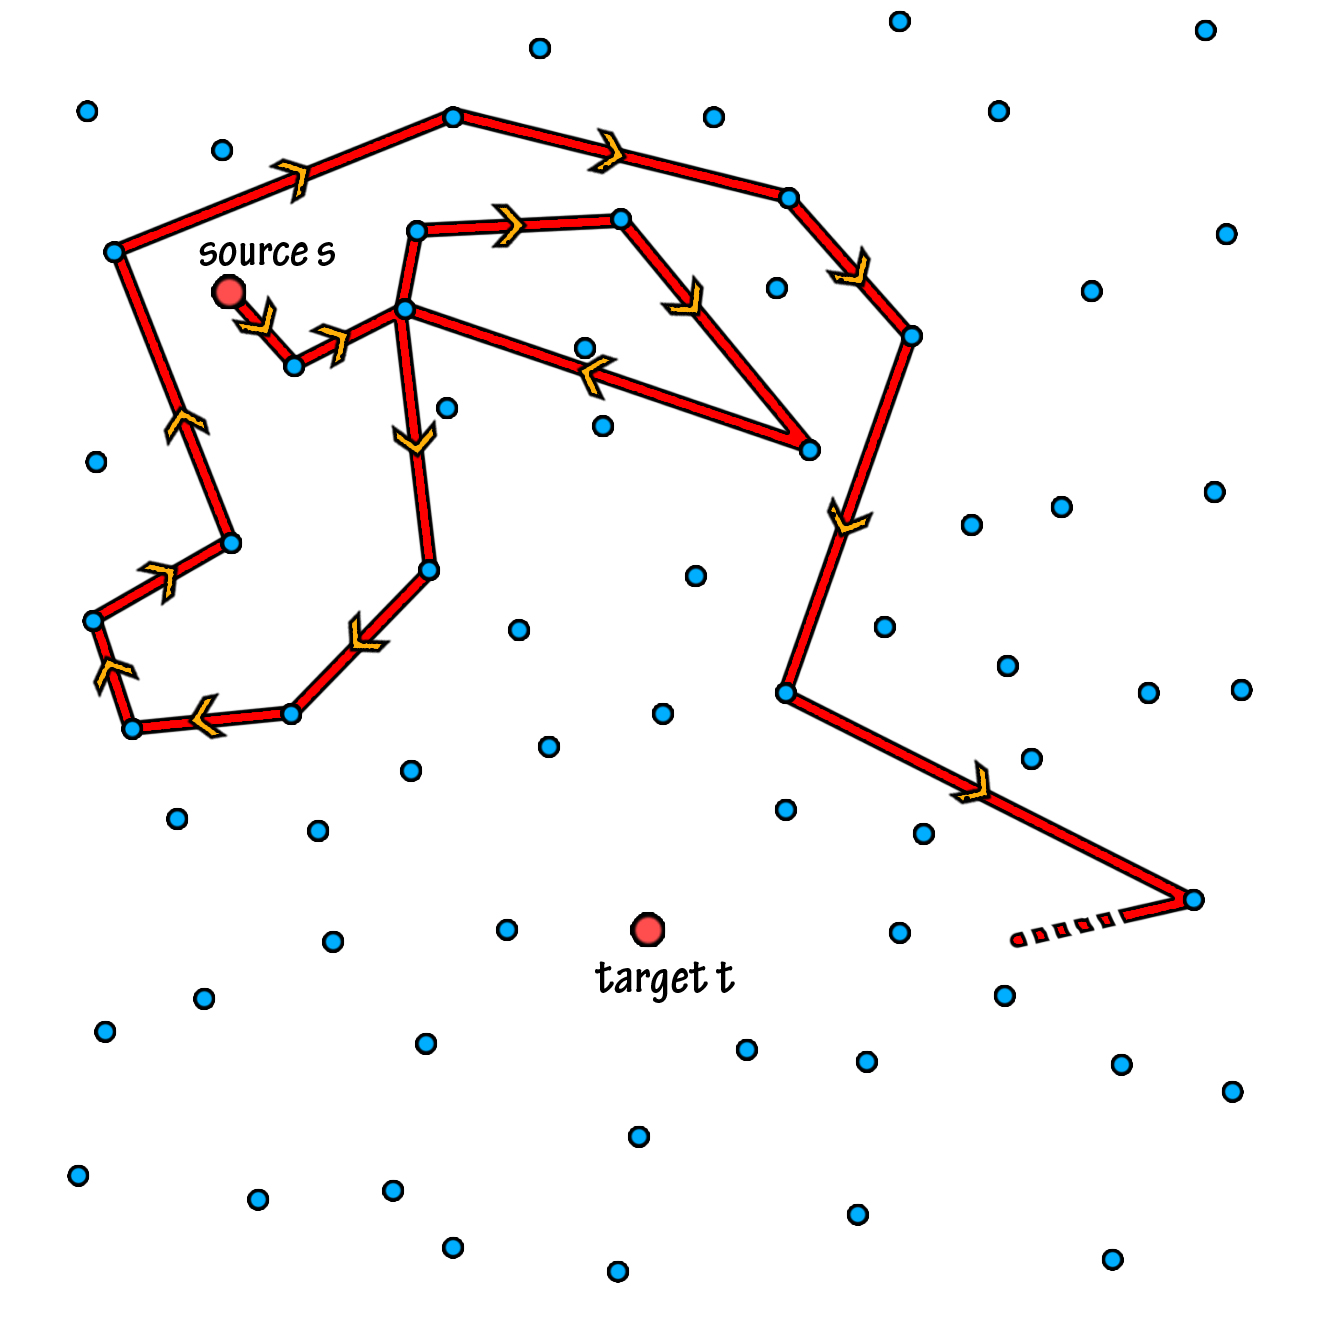
\includegraphics[scale=0.14]{Results/1rawrandomwalk.jpg}
\caption{1-way Random Walk}
\label{4_one_way}
\end{figure}

\subsubsection{2-Way Random Walk}

After taking random walks $W_s$ and $W_t$ from $s$ and $t$ simultaneously 
until the two walks intersect, one can find a path from $s$ to $t$.

This idea is similar to the one implemented in the learning phase in 
Section ~\ref{sec:4_learning_phase}. Let $\gamma_{s,t}$ denote the length of the path thus obtained. 
Let $\gamma$ be the average ratio of length of 2-way Random Walk and the 
length of the shortest path taken over all the unordered vertex pairs $(s,t)$, such that $s,t \in V$.


$$\gamma = \frac{1}{\left(\begin{array}{c} |V|\\ 2\end{array}\right)} \sum_{s,t \in V} \frac{\gamma_{s,t}}{d(s,t)}$$

Figure~\ref{4_two_way} illustrates the technique of 2-way random walk between $s$ and $t$. 
$W_s$ and $W_t$ are constructed simultaneously until they intersect.
The intersection point of the two walks is indicated by $H$. $W_s$ and $W_t$ 
are indicated by the red walk and green walk respectively. Source $s$ and the 
target $t$ are denoted by the red dots. 

\begin{figure}[htp]
\centering
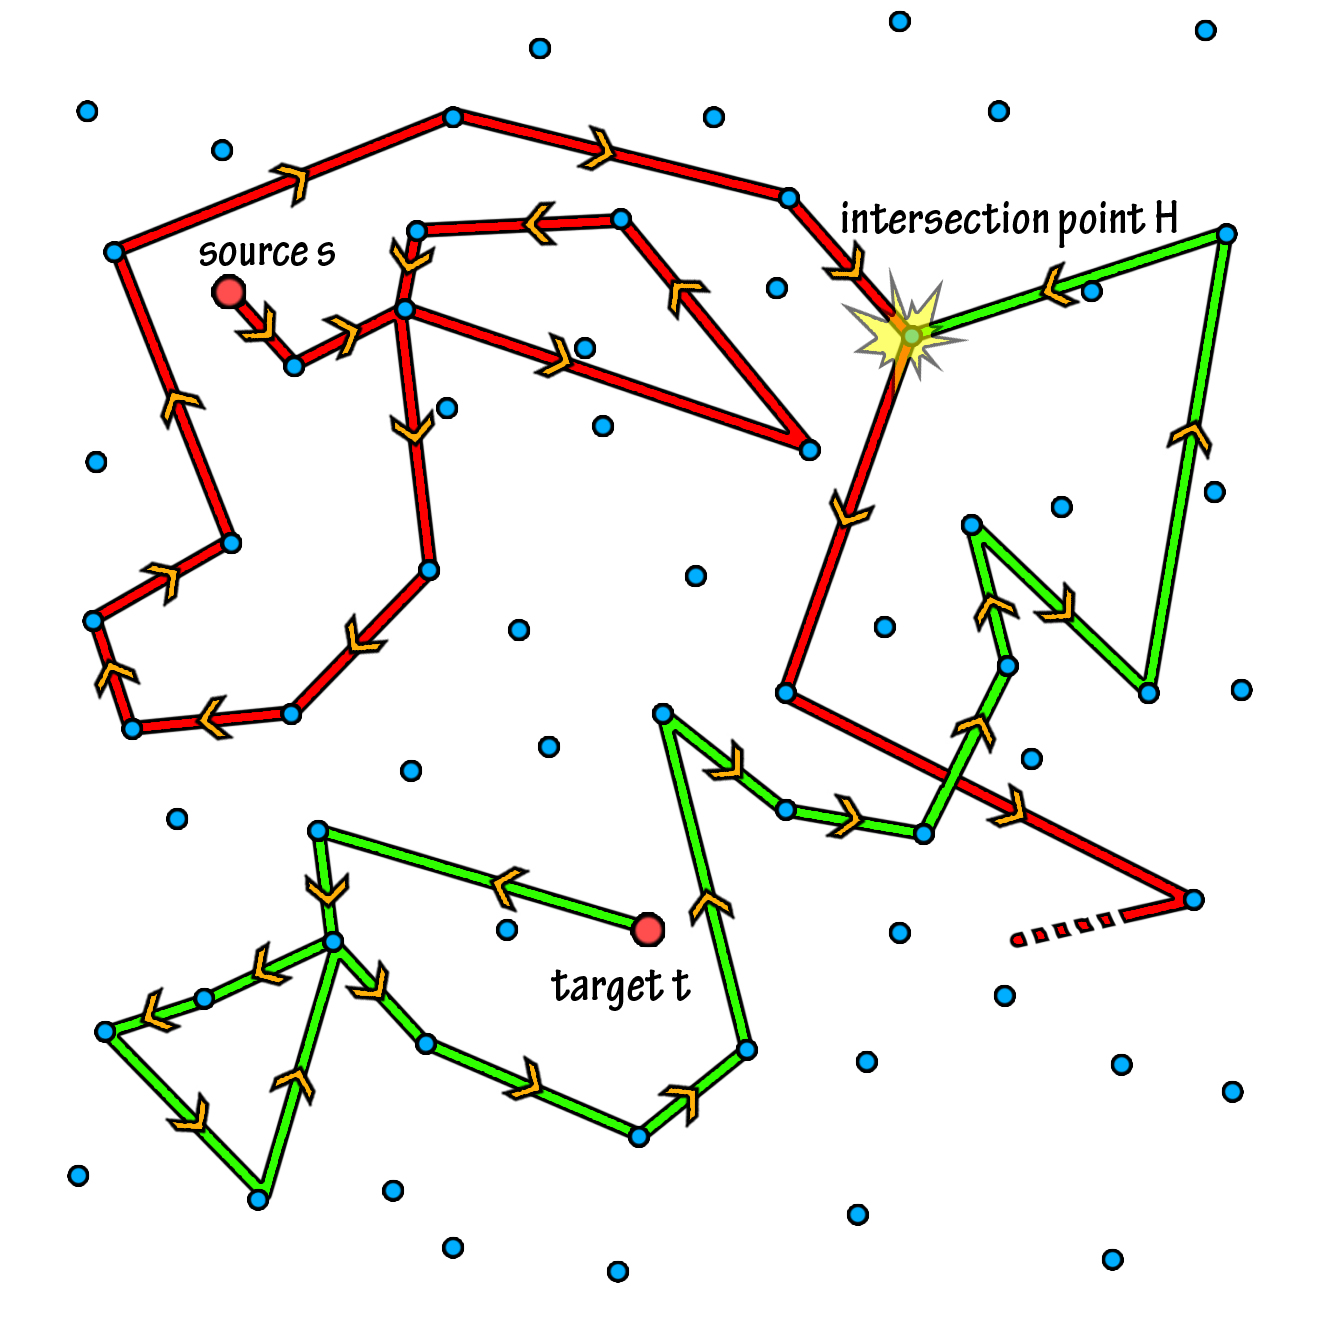
\includegraphics[scale=0.15]{Results/2rawrandomwalk.jpg}
\caption{2-Way Random Walk}
\label{4_two_way}
\end{figure}

\subsection{Comparison between PCA and Degree Based Navigation (Lada A. Adamic)}
Degree based navigation assumes that we have only local knowledge of the network. 
To pass a message from a source to a target, the source node passes the message to the neighbor with the highest degree. 
This process continues till the target is found. 
However, the message may not be passed to a node already visited, if it has other available neighbors. 
If there are no available neighbors, the message may be passed to a node that is already visited. 

\begin{figure}[htp]
\centering
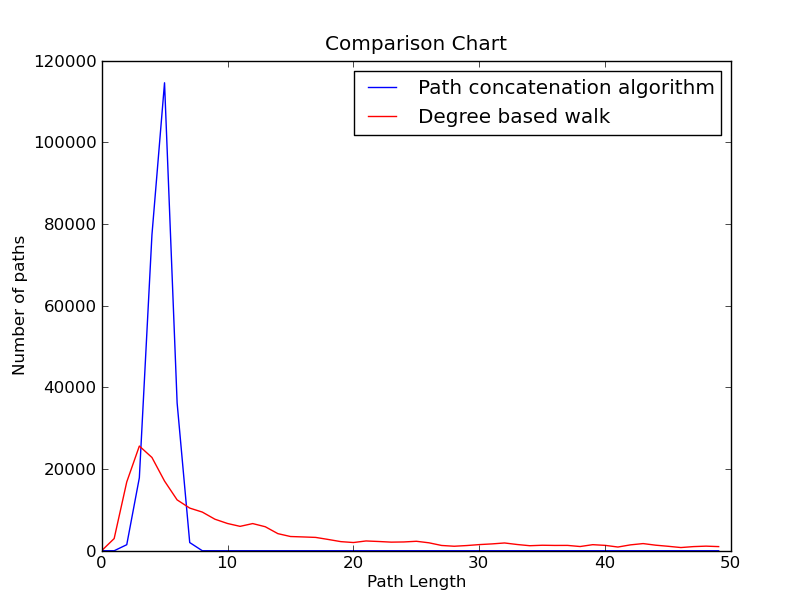
\includegraphics[scale=0.6]{Results/ADAMIC2.png}
\caption{Comparison between PCA and Degree Based Navigation}
\label{pca_vs_adamics}
\end{figure}

We compare the path lengths obtained from this type of navigation to the path lengths obtained using PCA for a Scale-Free network of 500 nodes, considering all the vertex pairs. Figure~\ref{pca_vs_adamics} illustrates the empirical results that we have obtained.The average path length for PCA and degree based navigation was found to be 4 and 24 respectively.

As evident from the plot, degree based navigation yields paths of much greater lengths than the PCA paths. 
This is due to the fact that the degree based approach spends a lot of hops between nodes of high degree during a brief initial period of exploring fresh nodes. 

\subsubsection{Path Concatenation Algorithm}
Let $\delta_{s,t}$ denote the length of the path from $s$ to $t$ obtained after 
executing the path concatenation algorithm. Let $\delta$ be the average ratio of 
length of the path obtained by the path concatenation algorithm and the length 
of the shortest path, taken over all the unordered vertex pairs $(s,t)$, such 
that $s,t \in V$.

$$\delta = \frac{1}{\left(\begin{array}{c} |V|\\ 2\end{array}\right)} 
\sum_{s,t \in V(G)} \frac{\delta_{s,t}}{d(s,t)}$$


\begin{figure}[htp!]
\centering
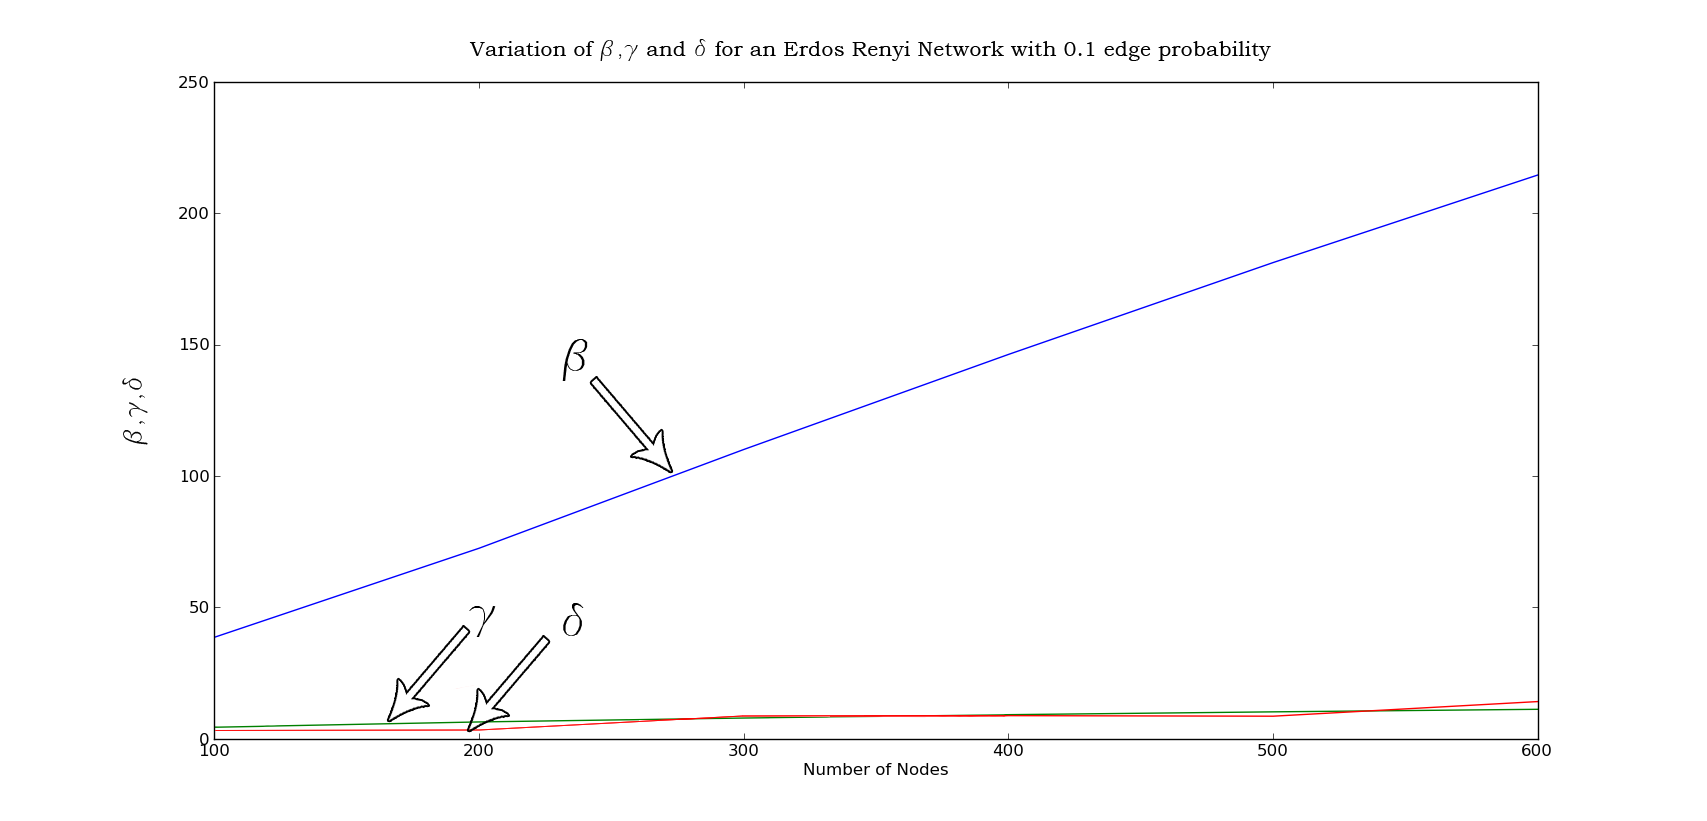
\includegraphics[scale=0.35]{Results/WalkComparisonErdos10.png}
\caption{Plot of $\beta$, $\gamma$ and $\delta$ 
versus the number of vertices for an Erdos-Renyi network with an edge probability of 0.1}
\label{4_performance_er}
\end{figure}

\begin{figure}[htp!]
\centering
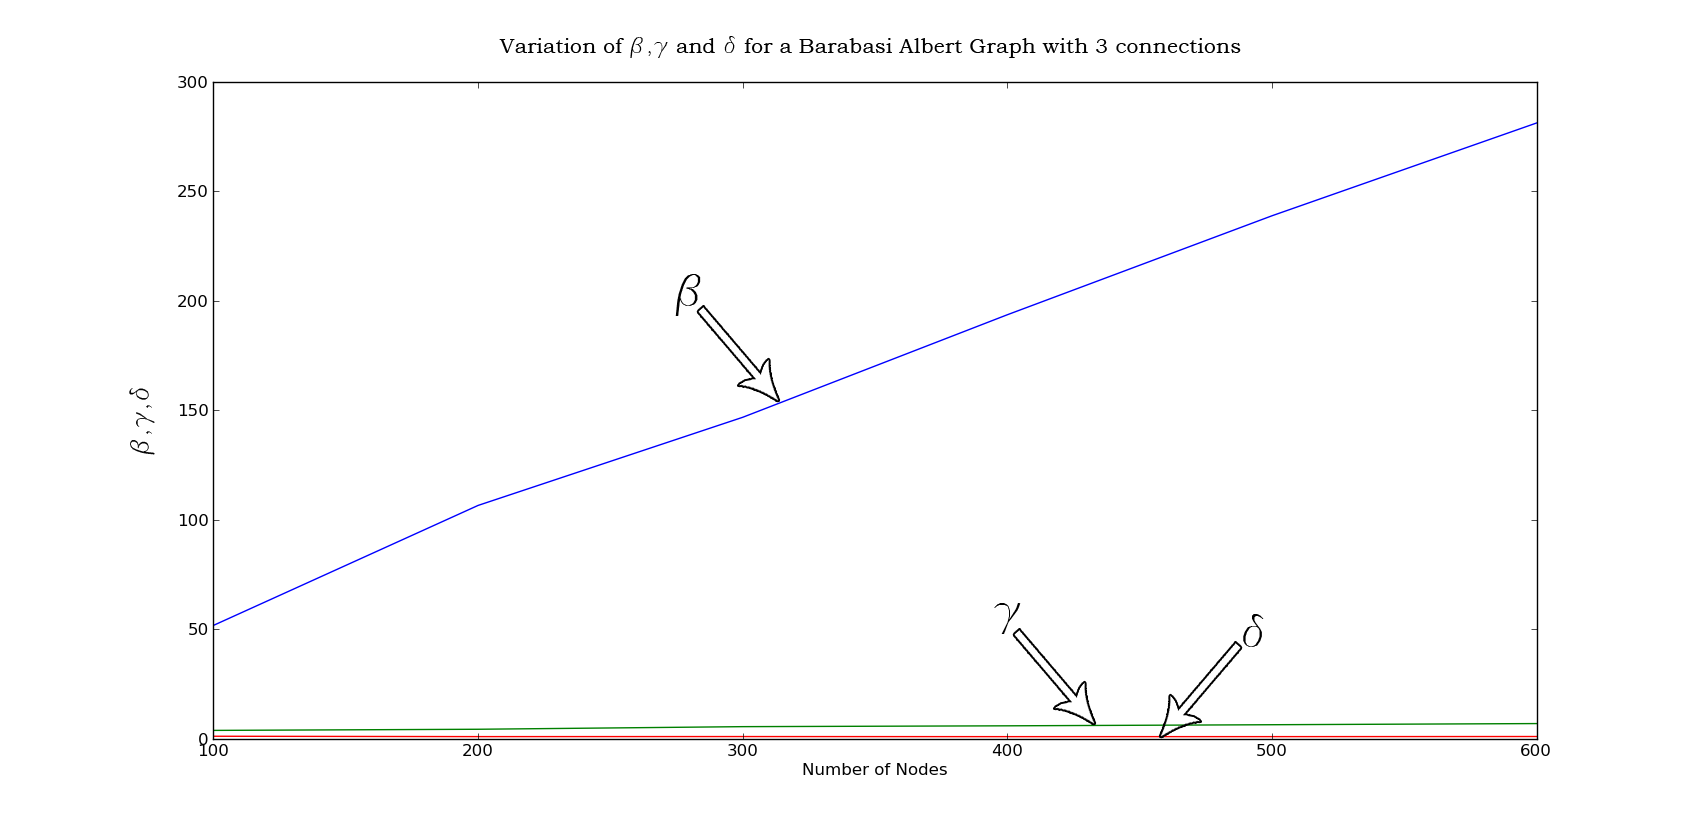
\includegraphics[scale=0.35]{Results/WalkComparisonBarabasi3.png}
\caption{Plot of $\beta$, $\gamma$ and $\delta$ versus the number
of vertices for a Barabasi-Albert Graph with 3 connections}
\label{4_performance_ba}
\end{figure}

\begin{figure}[htp!]
\centering
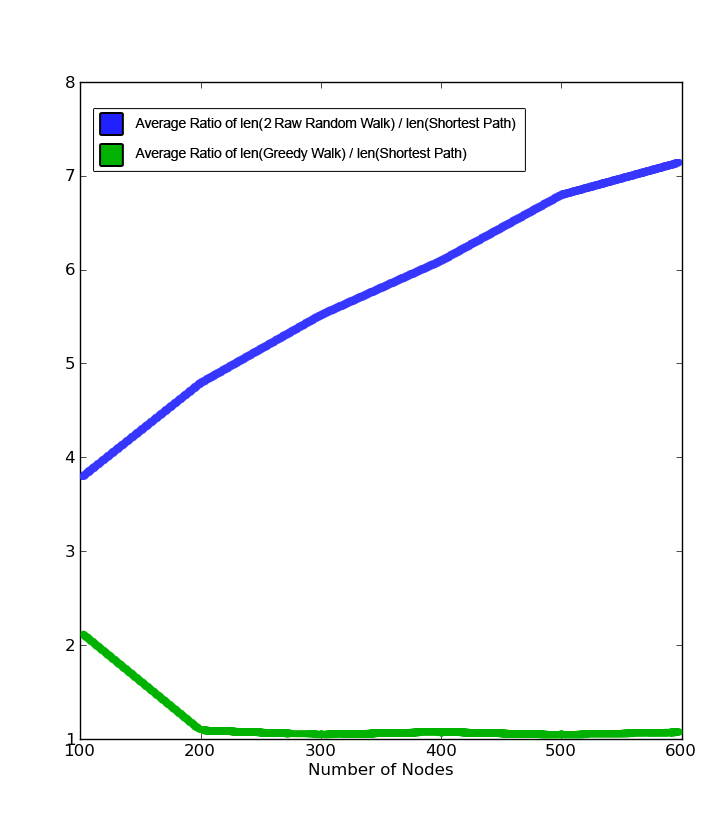
\includegraphics[scale=.4]{Results/barabasi4connections2raw.jpg}
\caption{This plot is a zoomed version of previous plot in 
Figure.~\ref{4_performance_ba} of  $\gamma$ and $\delta$ versus the number
of vertices for a Scale-free Graph with 4 connections}
\label{4_performance_ba_zoom}
\end{figure}


Figure.~\ref{4_performance_er} is a plot of variation of $\beta$, 
$\gamma$ and $\delta$ versus the number of vertices for an Erdos-Renyi network 
with an edge probability of 0.1. Figure.~\ref{4_performance_ba} is a plot of variation of 
$\beta$, $\gamma$ and $\delta$ versus the number of vertices for a 
scale free network with 4 connections. The blue curve indicates $\beta$, green curve 
indicates $\gamma$ and the red curve indicates $\delta$. From the plots, it is clear 
that the $\delta$-curve always lies below the $\beta$ curve. This implies that, the 
greedy navigation performs better than 1-way Random Walk.

In case of Erdos-Renyi networks, the $\delta$ curve and the $\gamma$ curve lie very 
close to each other, and also intersect at certain points in the plot. Hence, the 
performance of the proposed algorithm is as good as a 2-way random walk technique.

In case of scale-free graphs, the $\delta$ curve always lies below that 
of the $\gamma$ curve. Hence, the performance of the greedy technique is better than 
that of the 2-way random walk technique.



\subsection{Hotspot Distribution for Erdos-Renyi and Scale-free graphs}

The hotspot set we introduced exhibit some characteristic features. We note that 
the proposed path concatenation algorithm doesn't perform significantly 
better than the 2-way random walk. The reason being that the Erdos-Renyi graphs do not 
contain vertices of comparatively higher degree than the rest of the vertices in the graph. 
Whereas in case of a scale-free graph, some vertices have very high degree (\emph{hubs})
while the rest have comparatively low degree. These \emph{hubs} form valid candidates for 
the hotspot set. They can be reached in a few hops from any vertex in the graph, 
thus making the PCA an efficient strategy.


\begin{figure}[htp]
 
\begin{center}
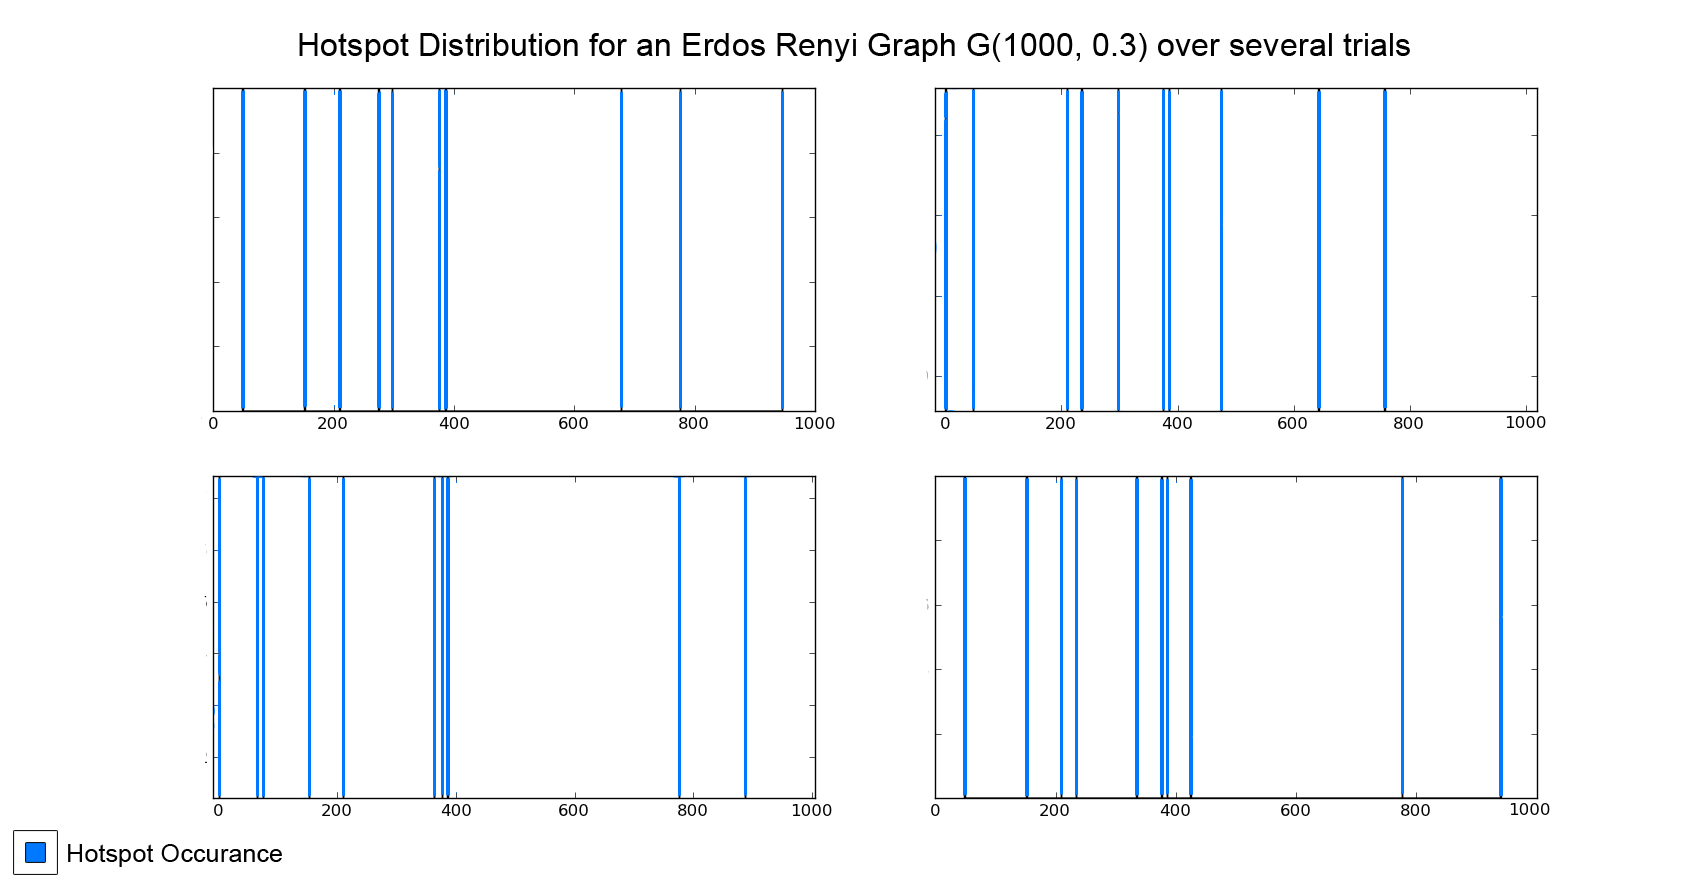
\includegraphics[scale=0.35]{Results/erdos.png}
\caption{Hotspot Distribution for an Erdos-Renyi Graph}
\label{4_hotspot_er}
\end{center}

\end{figure}



\begin{figure}[htp]
\begin{center}
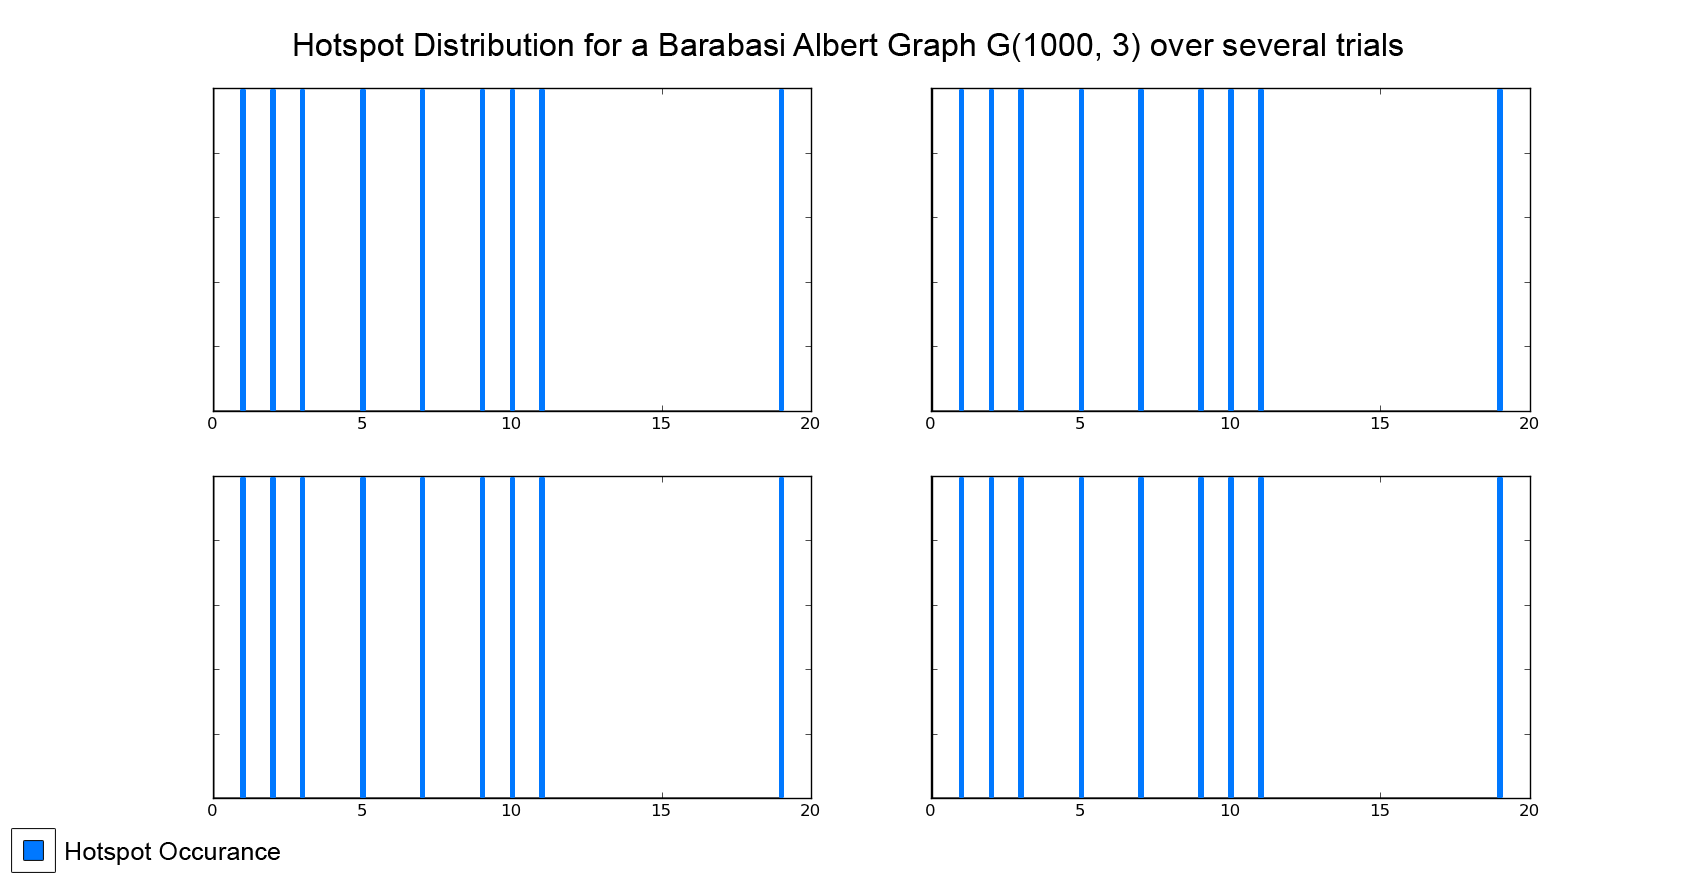
\includegraphics[scale=0.35]{Results/barabasi.png}\\
\caption{Hotspot Distribution for a Scale-free Graph}
\label{4_hotspot_ba}
\end{center}
\end{figure}

Fixing an Erdos-Renyi graph $G$ on 1000 vertices with probability 
$p=0.3$, as we run the learning phase of the PCA algorithm 4 times on the same graph, 
we note that the hotspot sets are different each time we run the algorithm. 
The top hotspot set is shown in Figure.~\ref{4_hotspot_er}, the x-axis denotes the vertex name 
and the vertical lines represent the hotspot. E.g. if a vertex, say 306, 
has a vertical line, it means that the vertex is chosen as a hotspot. 

Repeating the same procedure on a scale-free graph, we note that the top hotspot set
remains more or less the same as shown in Figure.~\ref{4_hotspot_ba}

\subsection{Center-strategic Paths on Scale Free Networks}

Given a path $(v_1,v_2,v_3,...,v_k)$ with closeness centrality 
values $(c_C(v_1),c_C(v_2),...,c_C(v_k))$ as defined in Section. \ref{sec:4_notions},
we compute the ranking of vertices $(R(v_1),R(v_2),R(v_3),...,R(v_k))$. By 
\emph{rank-plot} of this path, 
we mean a plot of the ranks $(R(v_1),R(v_2),R(v_3),...,R(v_k))$. 
If the rank-plot of a path has no more than one maxima, we call such a path 
a \emph{center-strategic path}. 

The algorithm presented in this article is inspired by the strategy
adapted by humans to learn the centers of a network and navigate in a 
center-strategic way. The presented algorithm resonates with the technique used 
by humans. We establish this fact by showing that the PCA algorithm yields 
center-strategic paths on scale free networks.

\begin{figure}[htp!]
 
\begin{center}
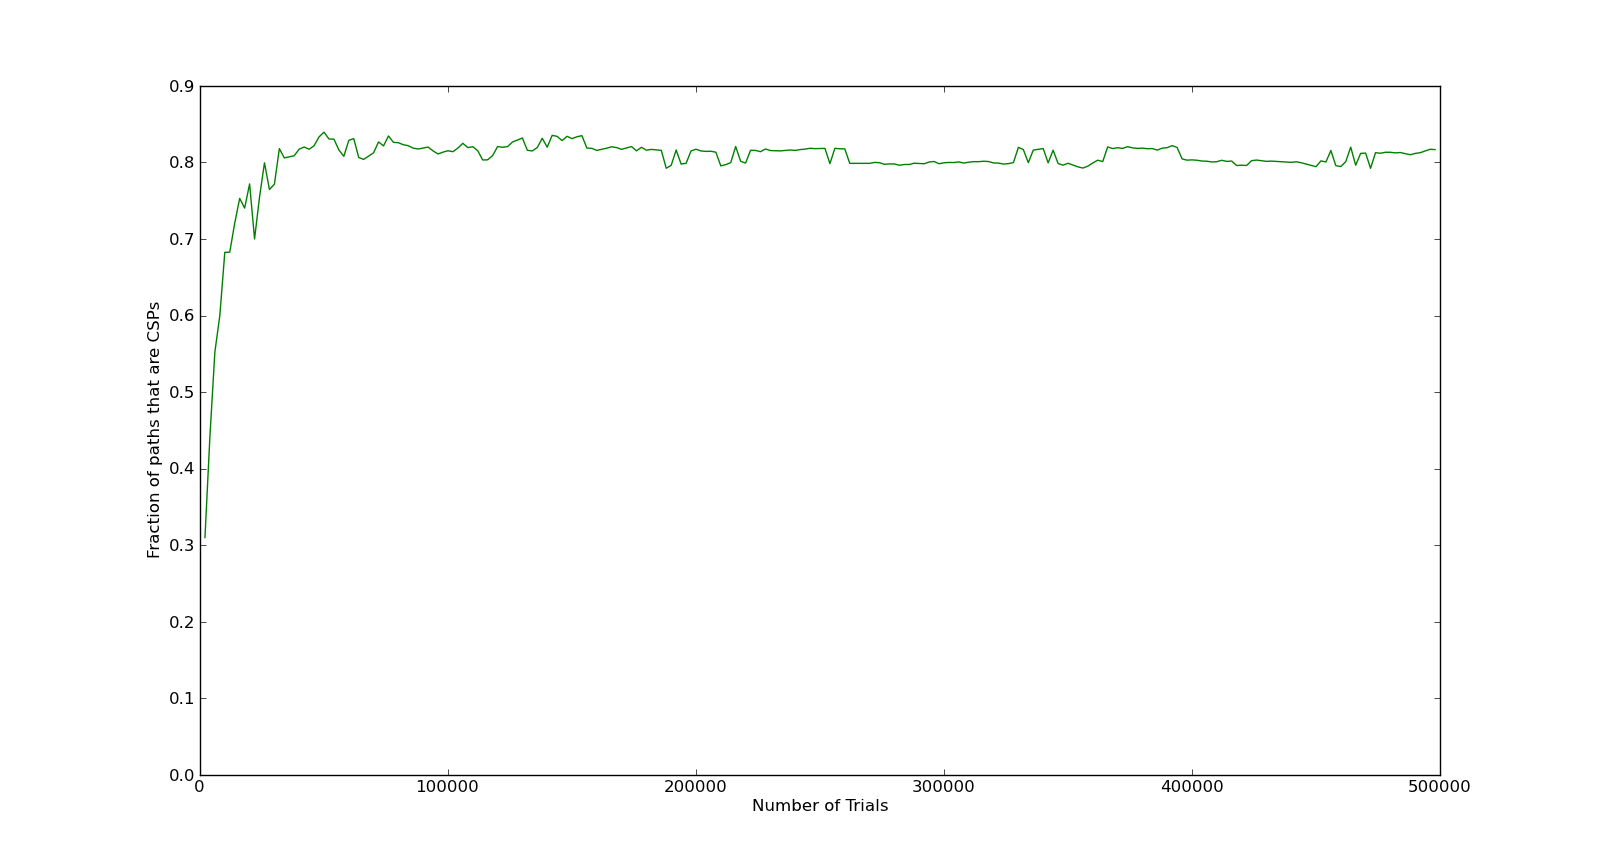
\includegraphics[scale = 0.35]{Results/barabasi_csp.png}
\caption{Center Strategic Paths Using Path Concatenation Algorithm}
\label{4_mainplot}
\end{center}
\end{figure}

Consider a scale-free graph $G(V,E)$. Let $k$ denote the number of iterations 
(or trials) during the navigation phase of the path concatenation algorithm.
After $k=100$, for every $k$, we jump to navigation phase, take $^{|V|}C_2$ greedy 
traversals (as explained in Section.~\ref{sec:4_navigation_phase}) between all vertex pairs and check for 
the number of paths that are center-strategic. The ratio of the number of 
center-strategic paths to the number of greedy traversals $^{|V|}C_2$ is denoted 
by $\psi$.

Figure.~\ref{4_mainplot} shows the variation of $\psi$ as k increases. We note that the path 
concatenation algorithm yields center-strategic paths 80\% of the times on 
scale free networks.

\newpage
\section{Implementation}
\begin{itemize}
 \item The above algorithm has been implemented using Python 2.7. 
 \item Python Development Kits used :
 \begin{itemize}
  \item NetworkX
  \item Matplotlib
  \item Numpy
  \item Scipy
  \item Pickle  
  \item Random
 \end{itemize}
\item yEd network visualization tool from yWorks.
\\\emph{http://www.yworks.com/en/products\_yed\_download.html}
\end{itemize}

 

\section{Conclusion}
\label{sec:4_conclusion}

Motivated by the strategy adopted by humans to navigate in an unknown environment, we presented
in this paper, an algorithm which simulates human navigation. We showed that the algorithm
performs better than the 1-way and 2-way random walk technique. We further showed that 
the proposed algorithm generates center-strategic paths on scale-free networks. 

A possible further work would be to study the convergence of the learning phase of 
the algorithm. One can start with the basic graph structures like the paths, grids, trees 
and study the hotspot distribution. It would also be interesting to classify the networks
on which the algorithm performs well and those on which it does not. One can study the 
performance of PCA algorithm on real - world networks as compared to other other 
navigational techniques. 

\section{Future Enhancement}  
\begin{itemize}
 \item The complexity of this algorithm is $O(n^{2 + \Delta})$. We wish to mathematically model the algorithm.  
 \item The existing algorithm is being applied for static networks. We wish to extend the algorithm for dynamically changing networks.
 \item We wish to ponder upon some of the new techniques for network navigation. Some of these include 
  \begin{itemize}
    \item BFS tree traversal
    \item Minimum spanning tree traversal
    \item Degree based walk
  \end{itemize}
\end{itemize}

\newpage
\section{Screenshots}

\begin{figure}[htp]
\begin{center}
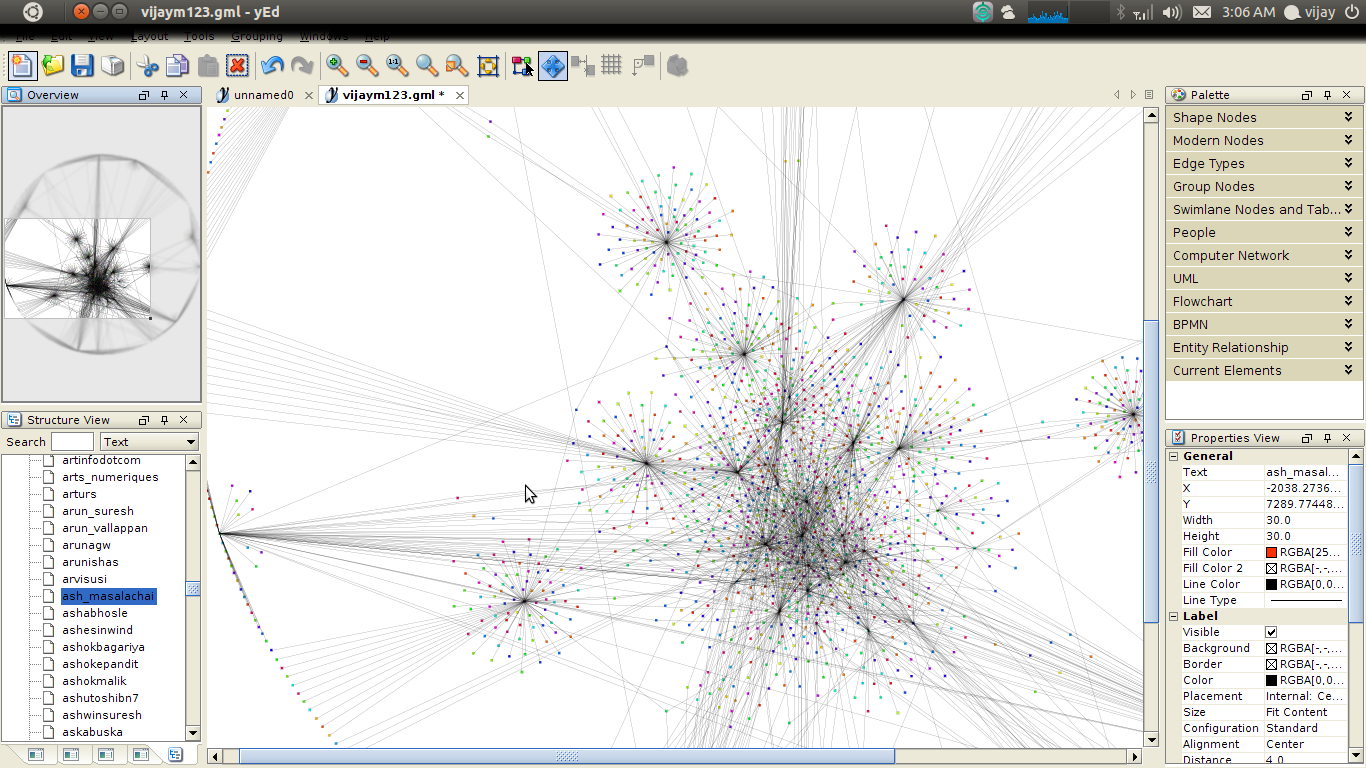
\includegraphics[scale = 0.30]{Results/yed.png}
\caption{Screenshots for yED}
\end{center}
\end{figure}

\begin{figure}[htp]
\begin{center}
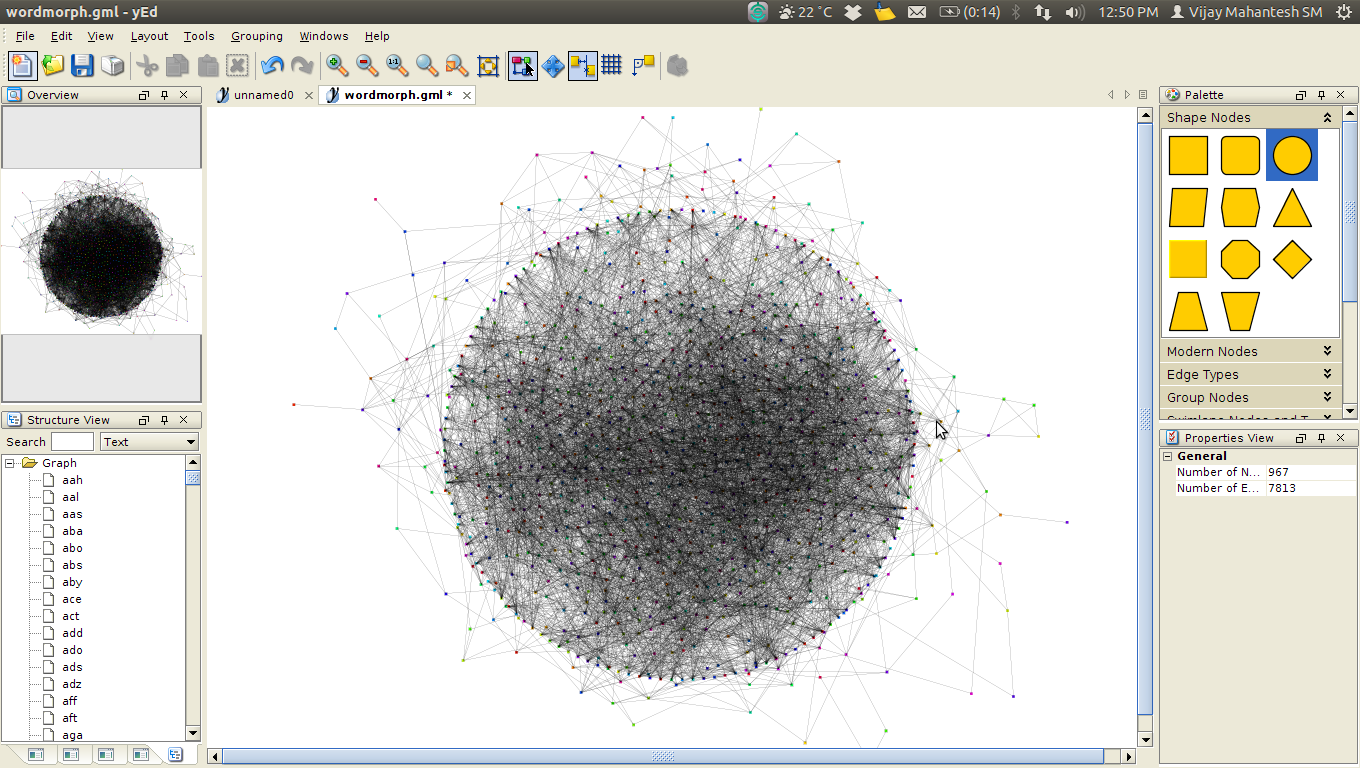
\includegraphics[scale = 0.29]{Results/WordMorpGame.png}
\caption{Screenshot of WordMorp Game Network.}
\end{center}
\end{figure}

\begin{figure}[htp]
\begin{center}
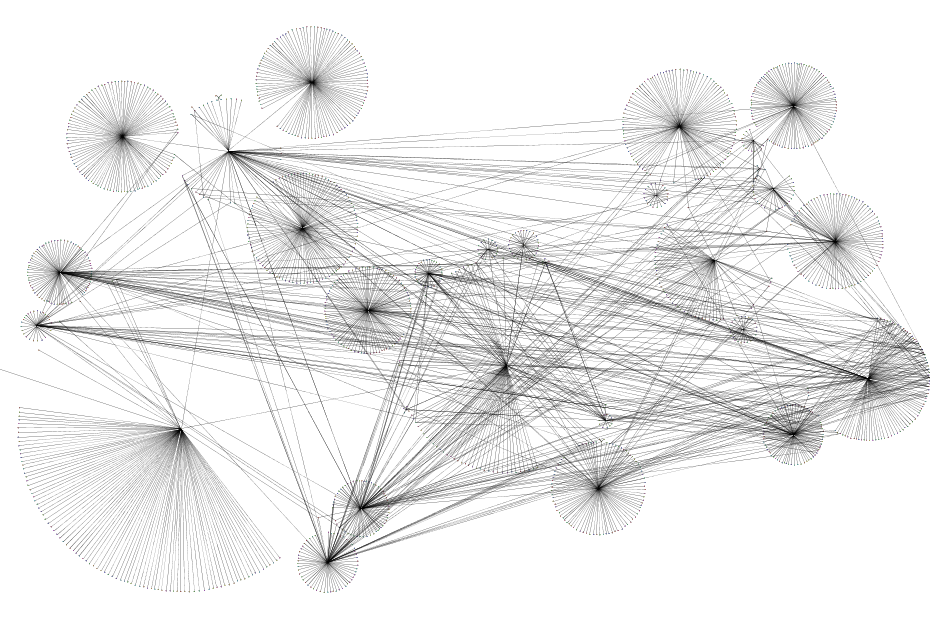
\includegraphics[scale = 0.28]{Results/Vijay_Twitter.png}
\caption{Twitter World Network upto 2 levels}
\end{center}
\end{figure}

\begin{figure}[htp]
\begin{center}
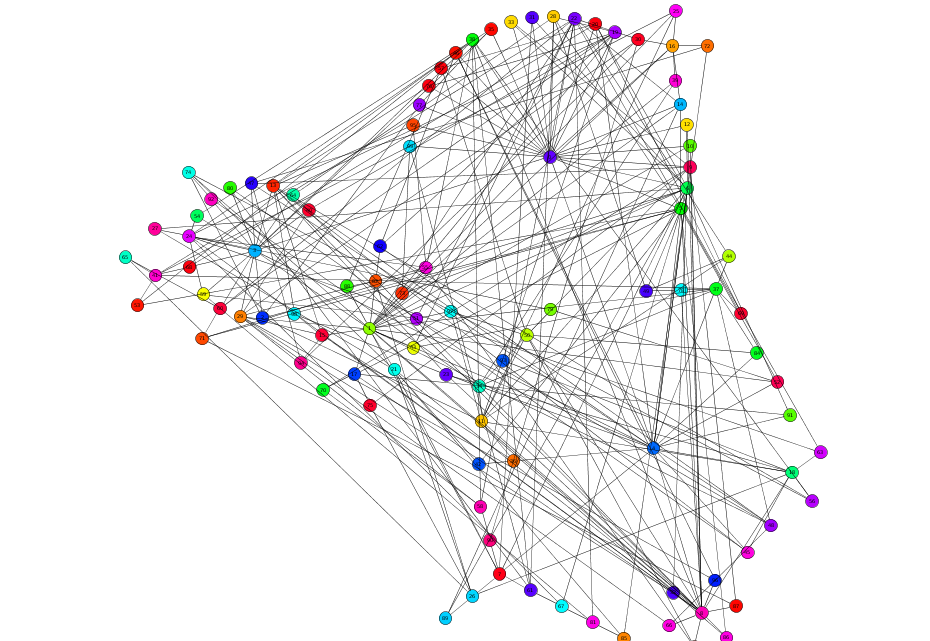
\includegraphics[scale = 0.28]{Results/barabasi_100_3.png}
\caption{Barabasi Network of 100 nodes and 3 connections.}
\end{center}
\end{figure}

\begin{figure}[htp]
\begin{center}
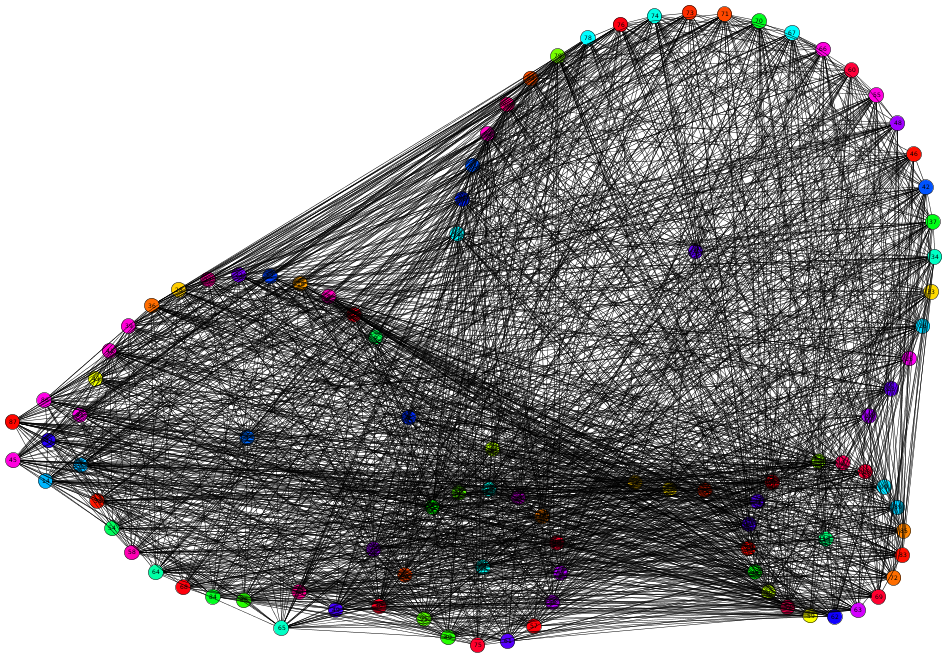
\includegraphics[scale = 0.28]{Results/erdos_renyi.png}
\caption{Erdos Renyi of 100 nodes of .4 probability.}
\end{center}
\end{figure}

\newpage                                                                                	
\bibliographystyle{plain}  
\bibliography{references}
\end{document}